\chapter{Étude préalable}
\fancyhead[L]{\leftmark}

%====================================================
\section{Introduction}

Ce chapitre constitue l'étude préalable du projet \textit{SecureRAG Hub}, plateforme de chatbots métiers sécurisés conçue dans le cadre d'un Projet de Fin d'Études du Master DSIR. Il poursuit quatre objectifs : (i)~situer le projet dans son contexte scientifique, fonctionnel et organisationnel~; (ii)~formuler la problématique, les questions de recherche et les hypothèses qui structurent le travail~; (iii)~préciser le périmètre, les objectifs et les contraintes de la solution~; (iv)~analyser les solutions existantes afin de justifier le positionnement retenu.

Le projet s'inscrit dans un contexte marqué par la diffusion rapide des modèles de langage de grande taille (LLM) et de l'intelligence artificielle générative dans les organisations. Selon le rapport \textit{AI Index} 2024, l'usage de l'IA générative s'est généralisé en moins de deux ans, tant dans les grandes entreprises que dans les administrations publiques, ce qui pose des défis inédits de gouvernance, de sécurité et d'audit \cite{stanford_ai_index_2024}. Les assistants conversationnels sont désormais perçus comme des leviers d'efficacité pour accéder à l'information, guider les utilisateurs et automatiser certaines interactions métier. Toutefois, leur intégration dans un environnement professionnel soulève des enjeux majeurs~: contrôle des accès, traçabilité des échanges, protection des données sensibles, gouvernance des modèles, fiabilité des réponses et maîtrise de la chaîne de déploiement. Ces enjeux sont notamment formalisés par la liste \textit{OWASP Top 10 for LLM Applications}, qui identifie les principales menaces propres aux applications fondées sur les LLM \cite{owasp_llm_top10}.

\textit{SecureRAG Hub} répond à cette problématique en proposant une plateforme intégrée et défendable. Le projet ne se limite pas à une interface conversationnelle~: il combine un portail web Laravel Blade, une architecture en microservices, une gouvernance par rôles, un socle Kubernetes local et une chaîne DevSecOps officielle pilotée par Jenkins. Cette orientation permet de présenter une solution démontrable, reproductible et alignée sur les exigences académiques d'un mémoire de niveau Master.

L'étude préalable poursuit donc un double objectif. D'une part, elle clarifie les besoins, les contraintes et les limites du projet. D'autre part, elle démontre que la valeur de la solution réside autant dans la gouvernance, la sécurité et l'industrialisation que dans la perspective d'intégration future d'un moteur d'intelligence artificielle complet de type \textit{Retrieval-Augmented Generation} (RAG).

Le chapitre est organisé comme suit. La section~\ref{sec:cadre_general} présente le cadre général du projet, la problématique, les questions de recherche, les hypothèses, les objectifs, le périmètre et les contraintes. La section~\ref{sec:cadre_acad} décrit le cadre académique et les parties prenantes. La section~\ref{sec:concepts} définit les concepts clés mobilisés. La section~\ref{sec:existant} analyse de manière critique les solutions existantes. La section~\ref{sec:solution} expose la solution proposée. La section~\ref{sec:methodologie} détaille le langage et la méthodologie de conception, ainsi que la démarche méthodologique de recherche. La section~\ref{sec:benefices} identifie les bénéfices attendus et les perspectives d'évolution. Une conclusion synthétise les apports du chapitre et annonce la suite du mémoire.

%====================================================
\section{Cadre général du projet}
\label{sec:cadre_general}

\subsection{Contexte et motivations}

\textit{SecureRAG Hub} est une plateforme unifiée de chatbots métiers sécurisés. Le projet est mené dans un cadre académique, au titre d'un Projet de Fin d'Études du Master DSIR. Il s'appuie sur des problématiques actuelles d'architecture logicielle, de sécurité applicative, de déploiement \textit{cloud-native} et d'intégration progressive de l'intelligence artificielle.

Dans de nombreuses organisations, les utilisateurs ont besoin d'accéder rapidement à des informations dispersées~: procédures de ressources humaines, assistance informatique, règles internes, consignes de sécurité ou documentation technique. Les chatbots métiers offrent une réponse intéressante à ce besoin grâce à leur interface simple et conversationnelle. Néanmoins, un chatbot d'entreprise ne peut être traité comme un simple outil de génération de texte~: il doit être gouverné, audité, sécurisé et intégré dans un processus de livraison maîtrisé. Ce constat est partagé par la communauté DevSecOps, qui recommande l'intégration de la sécurité tout au long du cycle de vie logiciel \cite{myrbakken_devsecops_2017,nist_ssdf_800218}.

Les motivations du projet sont les suivantes~:
\begin{itemize}
    \item proposer une interface utilisateur et administrateur claire pour gérer des chatbots métiers~;
    \item contrôler les accès au moyen d'une approche RBAC (\textit{Role-Based Access Control}) éprouvée \cite{sandhu_rbac_1996,nist_rbac_standard}~;
    \item préparer l'intégration future d'une architecture RAG sans dépendre d'un LLM réel pour la soutenance~;
    \item démontrer une architecture en microservices déployable localement sur Kubernetes~;
    \item industrialiser le projet par une chaîne DevSecOps vérifiable, en cohérence avec le cadre SLSA \cite{slsa_spec_v1}~;
    \item produire des preuves techniques exploitables dans un mémoire et lors d'une soutenance.
\end{itemize}

Cette combinaison rend le projet pertinent pour un Master DSIR car elle relie le développement applicatif, la sécurité, l'architecture distribuée, l'automatisation CI/CD et la documentation de preuve.

\subsection{Problématique et questions de recherche}

L'intégration de chatbots métiers dans un environnement professionnel soulève plusieurs difficultés conjuguées. Les réponses doivent être adaptées au domaine métier~; les utilisateurs ne doivent accéder qu'aux services autorisés~; les échanges doivent être tracés et auditables~; les déploiements doivent être reproductibles et vérifiables. À ces contraintes s'ajoute le risque spécifique aux systèmes d'intelligence artificielle générative~: une réponse peut paraître cohérente tout en étant inexacte, non sourcée ou inadaptée au contexte, phénomène désigné dans la littérature sous le terme d'\textit{hallucination} \cite{ji_hallucination_survey,bommasani_foundation_models}.

La difficulté centrale ne réside donc pas seulement dans la génération de réponses. Elle réside dans la capacité à \textit{encadrer} ces réponses, à \textit{gouverner} les usages, à \textit{sécuriser} la chaîne logicielle, à \textit{tracer} les opérations et à \textit{démontrer} que la plateforme effectivement déployée correspond à une version validée. Cette problématique articule trois préoccupations complémentaires bien identifiées dans la littérature : la sécurité applicative \cite{owasp_llm_top10}, la sécurité de la \textit{supply chain} logicielle \cite{slsa_spec_v1,ohm_supply_chain_attacks_2020} et l'industrialisation \textit{cloud-native} \cite{burns_kubernetes_2022}.

À partir de ces constats, la problématique centrale du mémoire est formulée de la manière suivante~:

\begin{quote}
\textbf{Comment concevoir, mettre en œuvre et valider une plateforme de chatbots métiers sécurisée, gouvernée par rôles, ouverte à une intégration RAG ultérieure, et industrialisée par une chaîne DevSecOps reproductible et auditable~?}
\end{quote}

Cette problématique se décline en trois questions de recherche (QR) opérationnelles~:

\begin{itemize}
    \item \textbf{QR1 — Architecture et gouvernance.} Quelle architecture logicielle (portail web, microservices, RBAC, base documentaire) permet de gouverner finement l'accès et l'usage de chatbots métiers tout en préservant la lisibilité et la maintenabilité de la solution~?
    \item \textbf{QR2 — Industrialisation DevSecOps.} Quels contrôles automatisés (analyse statique, détection de secrets, scan de vulnérabilités, génération de SBOM, signature et vérification d'images, politiques d'admission) doivent être intégrés à un pipeline CI/CD afin de produire des artefacts vérifiables et conformes aux bonnes pratiques de sécurité de la \textit{supply chain}~?
    \item \textbf{QR3 — Validation et reproductibilité.} Comment démontrer, par des preuves techniques reproductibles, que la plateforme déployée localement (mode \texttt{demo}) correspond bien à la version validée par le pipeline et à quels résultats mesurables est-il raisonnable de prétendre dans un cadre académique~?
\end{itemize}

\subsection{Hypothèses de recherche}

L'étude est structurée autour de trois hypothèses, qui guident les choix de conception et d'évaluation~:

\begin{itemize}
    \item \textbf{H1.} Une architecture en microservices Laravel exposant des API REST versionnées, couplée à un portail Blade, permet d'implémenter le RBAC et la gouvernance des chatbots métiers sans introduire de complexité disproportionnée par rapport à la valeur académique attendue.
    \item \textbf{H2.} L'intégration de Jenkins comme orchestrateur officiel, combinée aux outils Semgrep, Gitleaks, Trivy, Syft, Cosign et Kyverno, est suffisante pour atteindre un niveau de maturité DevSecOps compatible avec les exigences SLSA L2/L3 \cite{slsa_spec_v1} sur le périmètre réalisé en mode \texttt{demo}.
    \item \textbf{H3.} La séparation explicite entre les composants \textit{validés} (portail, microservices, sécurité du cluster) et les composants \textit{préparés mais non exécutés} (RAG, LLM, supply chain en mode \texttt{execute}) renforce la crédibilité scientifique du mémoire en distinguant rigoureusement les résultats démontrés des perspectives.
\end{itemize}

Ces hypothèses seront confrontées aux résultats expérimentaux dans les chapitres suivants, à travers les preuves générées par la chaîne d'outils (rapports de scan, SBOM, signatures, manifestes Kubernetes appliqués, rapports de validation finale).

\subsection{Objectifs du projet}

L'objectif général du projet est de \textbf{concevoir, implémenter et valider une plateforme académique de chatbots métiers sécurisée et industrialisée}, démontrable localement et préparée à une intégration RAG ultérieure. Cet objectif général se décline en objectifs spécifiques répartis sur trois dimensions complémentaires.

\paragraph{Dimension applicative.} Fournir un portail web Laravel Blade qui permet~:
\begin{itemize}
    \item l'accès différencié aux espaces utilisateur et administrateur~;
    \item la gestion des utilisateurs, des rôles et des permissions selon le modèle RBAC~;
    \item la gestion d'un catalogue de chatbots métiers (création, configuration, désactivation)~;
    \item la préparation des conversations et de leur historique~;
    \item la consultation d'informations de sécurité, d'audit et de supervision.
\end{itemize}

\paragraph{Dimension architecturale.} Structurer la plateforme afin de~:
\begin{itemize}
    \item décomposer le système en microservices à responsabilités clairement délimitées~;
    \item exposer des API REST versionnées (\texttt{/api/v1}) selon les bonnes pratiques OpenAPI~;
    \item isoler les responsabilités entre portail, services métiers, API Gateway et composants IA futurs~;
    \item préparer une intégration ultérieure avec un orchestrateur LLM et une base vectorielle.
\end{itemize}

\paragraph{Dimension DevSecOps.} Industrialiser le projet afin de~:
\begin{itemize}
    \item automatiser les tests, les analyses de qualité et les scans de sécurité dans un pipeline Jenkins~;
    \item utiliser Jenkins comme source officielle de CI/CD, avec GitHub Actions en miroir historique~;
    \item déployer le mode \texttt{demo} sur un cluster Kubernetes local (\texttt{kind})~;
    \item produire des preuves vérifiables de validation, de déploiement et de sécurité~;
    \item préparer une chaîne d'approvisionnement logicielle conforme à SLSA, intégrant SBOM CycloneDX, signature Cosign, vérification, promotion par digest et politiques Kyverno \cite{slsa_spec_v1,cyclonedx_spec,sigstore_paper}.
\end{itemize}

Ces objectifs sont formulés selon le critère SMART~: ils sont \textit{spécifiques}, \textit{mesurables} (chacun est associé à des artefacts ou indicateurs vérifiables), \textit{atteignables} dans la durée du PFE, \textit{réalistes} compte tenu des contraintes académiques, et \textit{temporellement délimités} par le calendrier des sprints (cf.\ section~\ref{sec:methodologie}).

\subsection{Périmètre et limites}

Le périmètre principal couvre la réalisation d'une plateforme démontrable de chatbots métiers sécurisée. Il inclut le portail Laravel Blade, les microservices métiers Laravel (auth-users, chatbot-manager, conversation-service, audit-security-service), le déploiement Kubernetes local, la chaîne Jenkins, les contrôles de sécurité automatisés et les artefacts de preuve associés.

Le projet ne vise pas, dans cette version, à entraîner un modèle d'intelligence artificielle, à développer un moteur RAG complet, ni à garantir l'exécution d'un LLM réel en production. Ces éléments constituent des perspectives d'évolution explicitement assumées. La version soutenue privilégie un scénario \texttt{demo} stable, dans lequel les composants IA sont représentés par des adaptateurs ou des services contrôlés.

Cette limite est volontaire et revendiquée. Elle permet de distinguer rigoureusement, conformément à l'hypothèse~H3~:

\begin{itemize}
    \item ce qui est effectivement opérationnel et validé (statut \texttt{TERMINÉ})~;
    \item ce qui est simulé pour garantir la stabilité de la démonstration (statut \texttt{PARTIEL})~;
    \item ce qui est prêt à être exécuté dans un environnement complet (statut \texttt{PRÊT\_NON\_EXÉCUTÉ})~;
    \item ce qui dépend d'un environnement externe non disponible en local (statut \texttt{DÉPENDANT\_DE\_L\_ENVIRONNEMENT}).
\end{itemize}

Cette taxonomie de statut est utilisée de manière cohérente dans l'ensemble du mémoire et des artefacts de validation.

\subsection{Contraintes du projet}

Le projet est soumis à plusieurs contraintes structurantes~:

\begin{itemize}
    \item maintenir un mode \texttt{demo} stable et reproductible sur un poste de développement standard~;
    \item éviter toute dépendance obligatoire à un modèle IA lourd ou à un service cloud payant~;
    \item ne jamais exposer de secrets réels dans le dépôt Git (gestion par variables d'environnement, fichiers chiffrés SOPS, ou \textit{External Secrets Operator})~;
    \item conserver une architecture lisible, modulaire et maintenable~;
    \item produire des preuves techniques vérifiables et archivées~;
    \item distinguer explicitement les éléments validés des éléments dépendants de l'environnement~;
    \item rester compatible avec la chaîne d'outils retenue~: Docker, \texttt{kind}, Kubernetes, Kustomize, Jenkins, Semgrep, Gitleaks, Trivy, Syft, Cosign et Kyverno.
\end{itemize}

Ces contraintes orientent fortement la conception. Elles expliquent notamment le choix d'un mode \texttt{demo} officiel, la séparation entre services applicatifs et composants IA, ainsi que l'importance accordée aux \textit{runbooks} et aux artefacts de validation archivés.

%====================================================
\section{Cadre académique et parties prenantes}
\label{sec:cadre_acad}

\subsection{Cadre académique du projet}

Le projet est mené dans un cadre académique. Dans l'état actuel du mémoire, il ne dépend pas d'un organisme d'accueil dont les informations seraient officiellement documentées~; afin d'éviter toute approximation, cette section présente le cadre fonctionnel et pédagogique du projet plutôt qu'une description institutionnelle non vérifiée.

\textit{Information à préciser par l'étudiant} : si un organisme d'accueil doit être ajouté dans la version finale, il conviendra d'y intégrer uniquement des informations confirmées (nom de l'organisme, domaine d'activité, missions, service d'affectation, encadrants, coordonnées et contexte exact du besoin).

\subsection{Parties prenantes fonctionnelles}

La plateforme cible plusieurs profils d'acteurs~:

\begin{itemize}
    \item les \textbf{utilisateurs métiers}, qui interagissent avec les chatbots autorisés selon leur domaine~;
    \item les \textbf{administrateurs plateforme}, responsables de la configuration générale et du catalogue de chatbots~;
    \item les \textbf{administrateurs sécurité}, chargés du suivi des incidents et des journaux d'audit~;
    \item l'\textbf{équipe DevSecOps}, responsable des pipelines, des scans, des déploiements et de la production de preuves~;
    \item le \textbf{jury de soutenance}, qui évalue la cohérence fonctionnelle, technique et méthodologique du projet.
\end{itemize}

L'identification des parties prenantes permet de clarifier les priorités~: la plateforme doit être utilisable, gouvernée, démontrable et documentée.

\subsection{Organisation fonctionnelle simplifiée}

L'organisation fonctionnelle du projet peut être représentée comme suit (figure~\ref{fig:organigramme_fonctionnel_securerag}).

\begin{figure}[htbp]
    \centering
    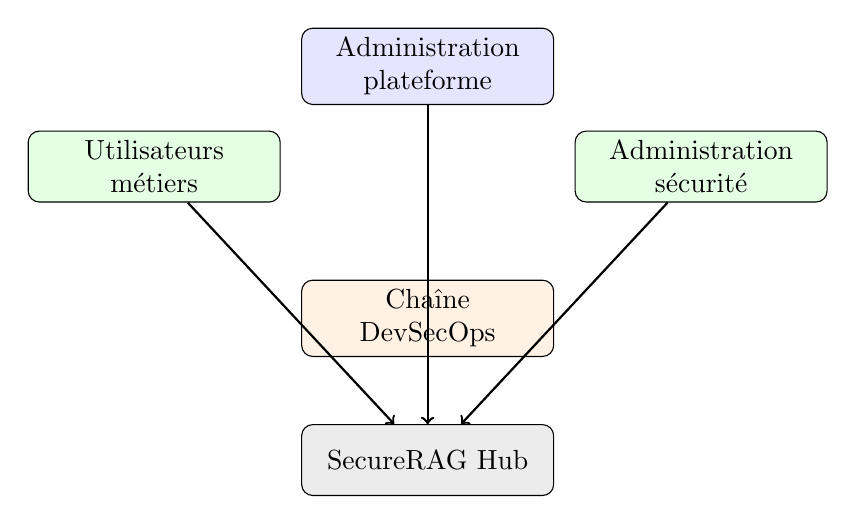
\begin{tikzpicture}[
        node distance=1.8cm,
        every node/.style={draw, rounded corners, align=center, minimum width=3.2cm, minimum height=0.9cm}
    ]
        \node[fill=blue!10] (admin) {Administration\\plateforme};
        \node[fill=green!10, below left of=admin, xshift=-2.2cm] (users) {Utilisateurs\\métiers};
        \node[fill=green!10, below right of=admin, xshift=2.2cm] (security) {Administration\\sécurité};
        \node[fill=orange!10, below of=admin, yshift=-1.4cm] (devsecops) {Chaîne\\DevSecOps};
        \node[fill=gray!15, below of=devsecops] (platform) {SecureRAG Hub};

        \draw[->, thick] (admin) -- (platform);
        \draw[->, thick] (users) -- (platform);
        \draw[->, thick] (security) -- (platform);
        \draw[->, thick] (devsecops) -- (platform);
    \end{tikzpicture}
    \caption{Organisation fonctionnelle simplifiée autour de SecureRAG Hub}
    \label{fig:organigramme_fonctionnel_securerag}
\end{figure}

%====================================================
\section{Concepts clés du projet}
\label{sec:concepts}

Cette section présente uniquement les notions strictement nécessaires à la compréhension de \textit{SecureRAG Hub}. L'objectif n'est pas de proposer un cours général sur l'intelligence artificielle ou Kubernetes, mais de définir les concepts directement mobilisés par le projet.

\subsection{Chatbot métier et plateforme sécurisée}

Un chatbot est un programme capable d'interagir avec un utilisateur via une interface conversationnelle. Un chatbot \textit{métier} se distingue d'un chatbot généraliste par son rattachement à un domaine précis~: ressources humaines, support informatique, sécurité, documentation interne ou assistance administrative.

Dans \textit{SecureRAG Hub}, le chatbot métier n'est pas seulement un canal de discussion. Il est associé à un domaine fonctionnel, à un niveau de sensibilité, à un ensemble de rôles autorisés, à une configuration de \textit{prompt} et à des règles de traçabilité. Cette approche, inspirée des bonnes pratiques de gouvernance des systèmes IA \cite{nist_ai_rmf_2023}, permet de traiter le chatbot comme une ressource gouvernée plutôt que comme une simple interface d'IA.

\subsection{Intelligence artificielle, apprentissage automatique et IA générative}

L'intelligence artificielle (IA) désigne un ensemble de techniques permettant à un système informatique d'accomplir des tâches qui requièrent habituellement des capacités humaines~: classification, prédiction, reconnaissance, analyse ou génération de contenu \cite{russell_norvig_ai}. L'apprentissage automatique (\textit{machine learning}) en constitue une branche majeure~: le système apprend à partir de données plutôt qu'à partir de règles entièrement explicites.

Trois familles d'apprentissage sont particulièrement utiles à situer. L'apprentissage supervisé utilise des exemples annotés pour apprendre à prédire une catégorie ou une valeur. L'apprentissage non supervisé recherche des structures dans des données non annotées, par exemple à travers le \textit{clustering}. L'apprentissage profond (\textit{deep learning}) repose sur des réseaux de neurones multicouches et constitue l'un des fondements des modèles de langage modernes \cite{russell_norvig_ai,goodfellow_deep_learning,lecun_deep_learning_2015}.

L'\textit{intelligence artificielle générative} est la branche qui produit du contenu à partir d'une requête~: texte, résumé, code, réponse conversationnelle ou aide à la décision. Les modèles de langage de grande taille (LLM) appartiennent à cette famille \cite{vaswani_transformer_2017,bommasani_foundation_models}. Ils peuvent générer des réponses cohérentes mais également produire des sorties erronées ou non vérifiées. Ce risque d'\textit{hallucination} \cite{ji_hallucination_survey} impose une gouvernance stricte dans un contexte professionnel, en cohérence avec les recommandations du NIST AI Risk Management Framework \cite{nist_ai_rmf_2023}.

Dans le projet, l'IA est traitée comme une capacité architecturale \textit{préparée}, et non comme un moteur complet déjà industrialisé. Le scénario officiel repose sur le mode \texttt{demo}, afin de démontrer la plateforme sans dépendre d'un LLM réel.

\subsection{RAG et base documentaire}

La génération augmentée par récupération, ou RAG (\textit{Retrieval-Augmented Generation}), combine une recherche documentaire avec une génération de réponse. Le système recherche d'abord des documents pertinents dans une base contrôlée (souvent au moyen de vecteurs sémantiques produits par un modèle d'\textit{embeddings}), puis transmet ces éléments à un modèle de langage chargé de produire une réponse contextualisée \cite{lewis_rag_2020,karpukhin_dpr_2020,gao_rag_survey_2024}.

Cette approche est particulièrement importante dans une plateforme métier, car elle réduit la dépendance aux connaissances générales du modèle et favorise des réponses fondées sur des sources internes maîtrisées. Elle nécessite généralement~: une base documentaire structurée, un modèle d'\textit{embeddings}, une base vectorielle (Qdrant, Milvus, pgvector ou équivalent) et un orchestrateur chargé de préparer le contexte transmis au LLM.

Dans \textit{SecureRAG Hub}, la logique RAG complète n'est pas implémentée dans la première version. La plateforme prépare cependant son intégration future grâce à une architecture séparant portail, API Gateway, microservices, orchestrateur LLM et service de connaissance, conformément à l'hypothèse~H3.

\subsection{RBAC et gouvernance des accès}

Le RBAC (\textit{Role-Based Access Control}) consiste à associer des permissions à des rôles, puis des rôles aux utilisateurs. Cette approche est formalisée depuis les travaux fondateurs de Sandhu \textit{et~al.} \cite{sandhu_rbac_1996} et standardisée par le NIST \cite{nist_rbac_standard}. Elle convient particulièrement aux plateformes multi-profils dans lesquelles différents acteurs (administrateur plateforme, administrateur sécurité, utilisateur RH, utilisateur IT) ne doivent pas disposer des mêmes droits.

Dans \textit{SecureRAG Hub}, les rôles structurants sont notamment \texttt{super-admin}, \texttt{admin-plateforme}, \texttt{admin-securite}, \texttt{user-rh} et \texttt{user-it}. Cette séparation gouverne l'accès aux utilisateurs, aux chatbots, aux conversations, aux incidents et aux preuves DevSecOps. Le RBAC s'applique simultanément au niveau applicatif (Laravel Policies, \textit{middleware} d'autorisation) et au niveau du cluster Kubernetes (Roles et RoleBindings).

\subsection{Architecture en microservices et API REST}

Une architecture en microservices décompose une application en services autonomes, chacun responsable d'un périmètre fonctionnel délimité \cite{newman_microservices,fowler_microservices_2014}. Cette organisation favorise la maintenabilité, l'évolutivité, la séparation des responsabilités et la possibilité de déployer indépendamment chaque service.

Dans le projet, les microservices couvrent l'authentification et le RBAC (\texttt{auth-users}), le catalogue de chatbots (\texttt{chatbot-manager}), les conversations (\texttt{conversation-service}), l'audit et la sécurité (\texttt{audit-security-service}). Les échanges sont structurés autour d'API REST versionnées sous le préfixe \texttt{/api/v1}. Cette convention facilite la stabilisation des contrats entre le portail Blade et les services métiers, conformément aux bonnes pratiques de l'OpenAPI Initiative \cite{openapi_spec}. La sécurisation des communications inter-services suit les recommandations du NIST SP~800-204 sur la sécurité des architectures microservices \cite{nist_sp_800_204}.

\subsection{Kubernetes, conteneurisation et déploiement local}

La conteneurisation permet d'embarquer une application et ses dépendances dans une image exécutable et portable. Docker est utilisé pour construire et lancer ces images. Kubernetes orchestre ensuite les conteneurs, gère les déploiements, les services, les volumes, les politiques réseau, les configurations et certaines capacités de résilience \cite{burns_kubernetes_2022,kubernetes_docs}.

Pour préserver la démontrabilité locale, \textit{SecureRAG Hub} utilise \texttt{kind} (\textit{Kubernetes in Docker}) afin de créer un cluster Kubernetes local reproductible \cite{kind_docs}. Les manifestes sont organisés avec Kustomize \cite{kustomize_docs} afin de séparer une base commune et des \textit{overlays} (\texttt{dev}, \texttt{demo}, \texttt{production}, \texttt{production-external-db}). Cette séparation, alignée sur les recommandations du \textit{CIS Kubernetes Benchmark} \cite{cis_k8s_benchmark}, permet de différencier explicitement les environnements et de tracer leurs spécificités.

\subsection{DevSecOps et chaîne d'approvisionnement logicielle}

Le terme DevSecOps désigne l'intégration continue de la sécurité dans le cycle DevOps \cite{myrbakken_devsecops_2017,humble_continuous_delivery}. La sécurité ne constitue plus un contrôle final, mais un ensemble de vérifications intégrées dès le code source, puis lors des tests, des scans, de la construction des images, de la signature, du déploiement et de l'admission au cluster Kubernetes. Le NIST formalise ces pratiques dans le \textit{Secure Software Development Framework} (SSDF, SP~800-218) \cite{nist_ssdf_800218}.

Les attaques récentes contre la chaîne d'approvisionnement logicielle (Solarwinds, dépendances NPM compromises, etc.) ont mis en évidence la nécessité de garanties cryptographiques de bout en bout \cite{ohm_supply_chain_attacks_2020}. Le cadre SLSA (\textit{Supply-chain Levels for Software Artifacts}) propose une échelle progressive de niveaux de maturité (L1 à L4) pour structurer ces garanties \cite{slsa_spec_v1}. Les outils Sigstore et Cosign permettent la signature et la vérification cryptographique des images de conteneurs et des artefacts \cite{sigstore_paper}.

Dans \textit{SecureRAG Hub}, Jenkins constitue la source officielle de CI/CD. Les contrôles incluent~:
\begin{itemize}
    \item \textbf{Semgrep} pour l'analyse statique du code (SAST)~;
    \item \textbf{Gitleaks} pour la détection de secrets dans le dépôt~;
    \item \textbf{Trivy} pour l'analyse des vulnérabilités logicielles dans les dépendances et les images~;
    \item \textbf{Syft} pour la génération de SBOM au format CycloneDX \cite{cyclonedx_spec}~;
    \item \textbf{Cosign} pour la signature et la vérification des images~;
    \item \textbf{Kyverno} pour les politiques d'admission Kubernetes \cite{kyverno_docs}.
\end{itemize}

La promotion par \textit{digest} OCI permet de déployer l'image effectivement validée par le pipeline plutôt qu'une image reconstruite ou référencée par un simple \textit{tag}. Cette chaîne peut être résumée ainsi~:

\begin{center}
\texttt{code $\rightarrow$ tests $\rightarrow$ scans $\rightarrow$ build $\rightarrow$ SBOM $\rightarrow$ sign $\rightarrow$ verify $\rightarrow$ promote $\rightarrow$ deploy $\rightarrow$ validate}
\end{center}

La mise en place complète de cette \textit{supply chain} avancée dépend de l'environnement d'exécution (registre local, clés Cosign, Syft, Docker, cluster Kubernetes). Le mémoire distingue donc systématiquement les étapes effectivement validées, les étapes prêtes à être rejouées et les étapes dépendantes de l'environnement.

\subsection{Sécurité Kubernetes}

La sécurité Kubernetes repose sur plusieurs mécanismes complémentaires. Les \textit{NetworkPolicies} restreignent les communications entre pods. Les \textit{ResourceQuotas} et \textit{LimitRanges} encadrent l'utilisation des ressources. Les \textit{PodDisruptionBudgets} améliorent la disponibilité lors de perturbations planifiées. Les \textit{HorizontalPodAutoscalers} préparent l'élasticité, sous réserve que \texttt{metrics-server} fournisse les métriques nécessaires. Les \textit{Pod Security Standards} (niveaux \texttt{privileged}, \texttt{baseline} et \texttt{restricted}) définissent les profils de sécurité applicables aux pods \cite{k8s_pod_security_standards}.

Kyverno permet d'ajouter des politiques d'admission à Kubernetes \cite{kyverno_docs}. En mode \texttt{Audit}, les ressources non conformes sont signalées sans être bloquées~; en mode \texttt{Enforce}, elles sont refusées par l'\textit{admission controller}. Pour un mémoire académique, il importe de présenter cette distinction avec rigueur, afin de ne pas confondre une politique \textit{prête à être appliquée} avec une politique \textit{réellement active en blocage}. Les bonnes pratiques de durcissement Kubernetes sont également formalisées dans le \textit{CIS Kubernetes Benchmark} \cite{cis_k8s_benchmark}.

\subsection{Technologies non retenues dans la version actuelle}

Certaines technologies pourraient apporter une valeur dans des contextes voisins mais ne sont pas retenues dans cette version du projet, afin de préserver la lisibilité de l'architecture~:
\begin{itemize}
    \item la \textit{blockchain}, qui peut être pertinente pour la traçabilité inter-organisationnelle, mais dont les besoins sont ici déjà couverts plus directement par les journaux d'audit, les digests OCI, les signatures d'images et les rapports Jenkins archivés~;
    \item les \textit{frameworks} d'agents avancés (LangGraph, AutoGen) qui, bien que prometteurs pour des cas d'usage RAG complexes, sont reportés en perspectives pour ne pas alourdir le périmètre du PFE~;
    \item les \textit{services managés cloud} (IAM cloud, KMS managé, registres managés), exclus pour respecter la contrainte de reproductibilité locale.
\end{itemize}

%====================================================
\section{Analyse et critique de l'existant}
\label{sec:existant}

\subsection{Critères d'analyse}

L'analyse de l'existant s'appuie sur les critères suivants, dérivés des questions de recherche QR1, QR2 et QR3~:
\begin{itemize}
    \item qualité de l'expérience conversationnelle~;
    \item gouvernance des accès (RBAC, audit, séparation des privilèges)~;
    \item intégration aux données internes et capacités RAG~;
    \item maîtrise de l'infrastructure et reproductibilité locale~;
    \item visibilité sur la chaîne DevSecOps (SAST, SBOM, signature, admission)~;
    \item ouverture (sources, formats, standards) et auditabilité~;
    \item contrainte de coût d'usage et indépendance vis-à-vis d'un fournisseur unique.
\end{itemize}

Ces critères permettent de comparer \textit{SecureRAG Hub} aux solutions commerciales et aux \textit{frameworks} techniques, sans prétendre rivaliser avec eux sur la puissance des modèles ou la maturité produit.

\subsection{Solutions commerciales orientées entreprise}

Plusieurs solutions commerciales ciblent désormais les organisations~: ChatGPT Enterprise, Microsoft Copilot Studio, Google Vertex~AI Agent Builder, Amazon Q Business et IBM watsonx Assistant. Elles se distinguent par leur maturité, la qualité de l'expérience utilisateur, la richesse de leurs connecteurs, leurs capacités d'administration et leur intégration aux écosystèmes cloud ou bureautiques \cite{openai_chatgpt_enterprise,microsoft_copilot_studio,google_vertex_ai_agent_builder,aws_q_business,ibm_watsonx_assistant}.

Leurs points forts sont importants~: adoption rapide, modèles puissants, infrastructures robustes et effort de développement initial réduit. Elles conviennent particulièrement aux entreprises qui souhaitent consommer un service managé plutôt que construire une plateforme complète.

Toutefois, leurs limites apparaissent dans le cadre de ce projet académique. Elles dépendent fortement d'un fournisseur unique (\textit{vendor lock-in}), masquent une grande partie de la chaîne technique interne et ne permettent pas toujours de démontrer localement le cycle complet~: construction d'images, génération de SBOM, signature Cosign, vérification, promotion par digest, déploiement Kubernetes et collecte de preuves. Par ailleurs, leur coût d'usage peut s'avérer rédhibitoire dans un cadre pédagogique.

\textit{SecureRAG Hub} se positionne donc différemment. Il ne vise pas à proposer le meilleur modèle conversationnel, mais à démontrer une architecture maîtrisée, sécurisée, reproductible et explicable devant un jury.

\subsection{Frameworks et plateformes techniques}

Des solutions comme Rasa, Botpress, LangChain ou LangGraph répondent à des besoins plus techniques. Rasa et Botpress facilitent la construction d'assistants conversationnels personnalisés~; LangChain et LangGraph permettent de concevoir des \textit{workflows} LLM, des chaînes RAG et des orchestrations avancées \cite{rasa_docs,botpress_docs,langchain_docs,langgraph_docs}.

Leur principal atout est la flexibilité~: ils conviennent aux équipes souhaitant construire des agents ou des assistants sur mesure et offrent davantage de contrôle qu'une solution SaaS entièrement managée. Toutefois, ces outils ne fournissent pas, à eux seuls, une plateforme complète intégrant gouvernance, sécurité, RBAC, déploiement Kubernetes, signature d'images et preuve DevSecOps. Ce sont des briques susceptibles d'être intégrées dans une architecture plus large.

\textit{SecureRAG Hub} peut donc être compris comme une plateforme d'intégration autour de telles briques. Dans une version future, LangChain ou LangGraph pourraient enrichir l'orchestration IA, tandis que Rasa ou Botpress pourraient inspirer certains mécanismes conversationnels. Dans la version actuelle, ces composants demeurent des perspectives et non des dépendances centrales.

\subsection{Tableau comparatif synthétique}

Le tableau~\ref{tab:comparatif_existant} synthétise le positionnement comparé de \textit{SecureRAG Hub} sur les critères retenus.

\begin{table}[htbp]
    \centering
    \small
    \begin{tabular}{|p{3.4cm}|p{1.6cm}|p{1.8cm}|p{1.8cm}|p{1.8cm}|p{2.6cm}|}
        \hline
        \textbf{Critère} & \textbf{ChatGPT Entreprise} & \textbf{Copilot Studio} & \textbf{Vertex AI / Q / watsonx} & \textbf{Rasa / LangChain} & \textbf{SecureRAG Hub (présent travail)} \\
        \hline
        Qualité LLM & ++ & ++ & ++ & + & N.\,A.\ (mode \texttt{demo}) \\
        \hline
        RBAC interne fin & + & + & + & $\sim$ & ++ \\
        \hline
        Reproductibilité locale & -- & -- & -- & + & ++ \\
        \hline
        Pipeline DevSecOps audité & $\sim$ & $\sim$ & $\sim$ & -- & ++ \\
        \hline
        SBOM + signature & $\sim$ & $\sim$ & $\sim$ & -- & ++ \\
        \hline
        Indépendance fournisseur & -- & -- & -- & ++ & ++ \\
        \hline
    \end{tabular}
    \caption{Positionnement comparatif de SecureRAG Hub sur les critères de l'analyse de l'existant. Légende~: ++ très favorable, + favorable, $\sim$ partiel, -- limité, N.\,A.\ non applicable.}
    \label{tab:comparatif_existant}
\end{table}

\subsection{Positionnement de SecureRAG Hub}

L'analyse montre que les solutions existantes sont généralement fortes sur l'un des axes suivants~: puissance conversationnelle, intégration cloud, productivité de création d'agents, ou flexibilité de développement. En revanche, elles mettent moins l'accent sur une démonstration locale complète associant portail métier, microservices, RBAC, Kubernetes, Jenkins, \textit{supply chain} et preuves vérifiables.

Le positionnement de \textit{SecureRAG Hub} est donc le suivant~:
\begin{itemize}
    \item offrir une plateforme académique \textit{complète} plutôt qu'un simple chatbot~;
    \item rendre explicite la gouvernance des utilisateurs, des rôles et des chatbots~;
    \item démontrer une architecture \textit{cloud-native} reproductible localement~;
    \item intégrer la sécurité dans la chaîne de livraison logicielle~;
    \item produire des preuves techniques exploitables en soutenance~;
    \item préparer l'intégration future du RAG sans la présenter comme déjà pleinement réalisée.
\end{itemize}

Cette position est défendable car elle évite une comparaison directe avec les grandes plateformes commerciales sur leur terrain principal. La valeur du projet réside dans la cohérence entre l'application métier, l'architecture distribuée, la sécurité et l'industrialisation.

%====================================================
\section{Solution proposée}
\label{sec:solution}

\subsection{Principe général}

La solution proposée, \textit{SecureRAG Hub}, est organisée en plusieurs couches (figure~\ref{fig:vue_simplifiee_securerag}). Le portail Laravel Blade constitue la surface utilisateur. Les microservices Laravel portent la logique métier. L'API Gateway prépare un point d'entrée technique unifié. Kubernetes exécute les composants conteneurisés. Jenkins orchestre la CI/CD et les validations de sécurité.

\begin{figure}[htbp]
    \centering
    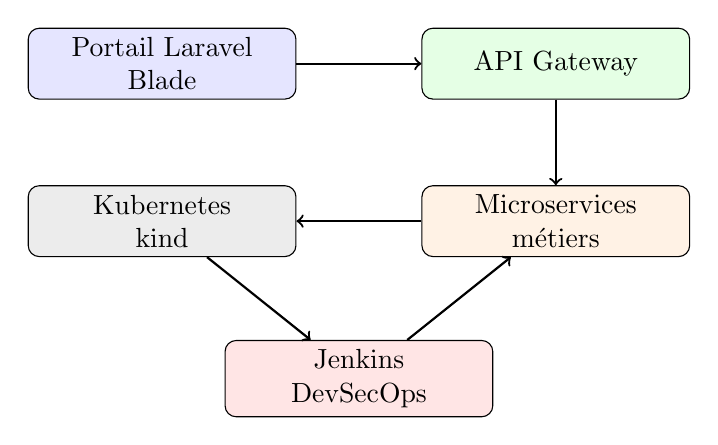
\begin{tikzpicture}[
        node distance=1.9cm,
        every node/.style={draw, rounded corners, align=center, minimum width=3.4cm, minimum height=0.9cm}
    ]
        \node[fill=blue!10] (portal) at (0,0) {Portail Laravel\\Blade};
        \node[fill=green!10] (gateway) at (5,0) {API Gateway};
        \node[fill=orange!10] (services) at (5,-2) {Microservices\\métiers};
        \node[fill=gray!15] (k8s) at (0,-2) {Kubernetes\\kind};
        \node[fill=red!10] (devsecops) at (2.5,-4) {Jenkins\\DevSecOps};

        \draw[->, thick] (portal) -- (gateway);
        \draw[->, thick] (gateway) -- (services);
        \draw[->, thick] (services) -- (k8s);
        \draw[->, thick] (k8s) -- (devsecops);
        \draw[->, thick] (devsecops) -- (services);
    \end{tikzpicture}
    \caption{Vue simplifiée de l'architecture SecureRAG Hub}
    \label{fig:vue_simplifiee_securerag}
\end{figure}

\subsection{Fonctionnalités prévues}

La plateforme regroupe les fonctionnalités suivantes~:
\begin{itemize}
    \item espace utilisateur permettant l'accès aux chatbots autorisés~;
    \item espace administrateur permettant de gérer utilisateurs, rôles et chatbots~;
    \item gestion du catalogue de chatbots métiers~;
    \item préparation des conversations et de leur historique~;
    \item supervision des incidents et consultation des preuves DevSecOps~;
    \item API REST destinées à connecter progressivement les écrans Blade aux services persistants.
\end{itemize}

\subsection{Choix techniques}

Laravel Blade est retenu pour le portail afin de réduire la complexité \textit{frontend} et de conserver une interface claire, maintenable et adaptée au périmètre académique. Vue.js et Inertia ne sont volontairement pas utilisés dans cette version, afin de respecter la contrainte de simplicité.

Laravel est également retenu pour les microservices métiers persistants, car il fournit un cadre robuste pour les migrations, les modèles Eloquent, les Form Requests, les Policies, les seeders et les tests automatisés. Des services FastAPI sont conservés à titre transitoire pour stabiliser le scénario de démonstration des composants IA, mais ils ne font pas partie du périmètre officiel pour la soutenance (cf.\ \texttt{docs/architecture/official-scope.md}).

Docker, \texttt{kind}, Kubernetes et Kustomize assurent la reproductibilité du déploiement. Jenkins constitue la source officielle de CI/CD, GitHub Actions étant conservé en miroir historique seulement. Les outils Semgrep, Gitleaks, Trivy, Syft, Cosign et Kyverno renforcent la dimension DevSecOps de la chaîne.

\subsection{Justification du mode demo}

Le mode \texttt{demo} est retenu comme scénario officiel de soutenance. Ce choix garantit une démonstration stable, contrôlée et indépendante d'un modèle IA lourd. Il permet également de présenter clairement l'état réel du projet~: le socle DevSecOps et Kubernetes est démontrable, les capacités IA sont préparées sur le plan architectural, et l'intégration RAG complète demeure une perspective explicite (hypothèse~H3).

Ce positionnement est important face au jury~: il évite de promettre un système IA complet alors que la valeur principale du projet tient dans la construction d'une plateforme sécurisée, industrialisée et prête à évoluer.

%====================================================
\section{Langage et méthodologie de conception}
\label{sec:methodologie}

\subsection{Démarche méthodologique de recherche}

Le mémoire adopte une démarche méthodologique de type \textit{recherche-action en ingénierie logicielle} \cite{wieringa_design_science_2014}. Cette démarche, dérivée du \textit{design science}, est particulièrement adaptée aux projets qui visent à concevoir un artefact (ici, la plateforme \textit{SecureRAG Hub}) tout en produisant des connaissances généralisables sur sa conception et sa validation.

L'approche retenue est qualitative et exploratoire, fondée sur~:
\begin{itemize}
    \item une phase d'\textbf{analyse} (revue de littérature et étude des solutions existantes)~;
    \item une phase de \textbf{conception} (architecture, modèles, choix techniques)~;
    \item une phase de \textbf{réalisation} itérative (sprints Scrum)~;
    \item une phase de \textbf{validation} par des artefacts vérifiables (rapports de scan, SBOM, signatures, manifestes appliqués, preuves Jenkins)~;
    \item une phase de \textbf{réflexion critique} sur les résultats obtenus, les limites et les perspectives.
\end{itemize}

L'évaluation s'appuie sur des critères techniques objectifs (taux de couverture des tests, nombre de vulnérabilités détectées, conformité Kyverno, succès des cycles \textit{build $\rightarrow$ sign $\rightarrow$ verify $\rightarrow$ deploy}), complétés par une analyse réflexive documentée. Aucune enquête par questionnaire ni étude utilisateur n'est réalisée dans ce travail~; ces dimensions appartiennent aux perspectives.

\subsection{Méthodologie Scrum}

Au sein de la phase de réalisation, le projet adopte une démarche agile inspirée de Scrum \cite{schwaber_scrum_guide}. Ce choix se justifie par la diversité des composants à réaliser~: portail web, API, microservices, Kubernetes, sécurité, CI/CD, documentation et preuves de soutenance. Une approche strictement séquentielle aurait été peu adaptée, plusieurs contraintes ayant évolué au cours du projet (stabilité du mode \texttt{demo}, accès à GitHub depuis Jenkins, exécution complète de la \textit{supply chain}).

Scrum repose sur trois piliers utiles dans ce contexte~: transparence, inspection et adaptation. La \textit{transparence} consiste à documenter l'état réel du projet, sans masquer les limites. L'\textit{inspection} consiste à valider chaque incrément par des tests, des scans ou des commandes reproductibles. L'\textit{adaptation} consiste à ajuster les priorités lorsque l'environnement impose des contraintes (par exemple, indisponibilité d'un registre privé). Ce dernier point est fondamental pour préserver la cohérence académique du projet.

Chaque sprint devait produire un livrable vérifiable~: un écran, une API, un script, un manifeste Kubernetes, un rapport de scan, un \textit{support pack} ou une section du mémoire. Cette logique a permis d'éviter une progression purement théorique. Le tableau~\ref{tab:sprints_securerag} récapitule l'application progressive de Scrum.

\begin{table}[htbp]
    \centering
    \begin{tabular}{|p{2.2cm}|p{5.2cm}|p{6.2cm}|}
        \hline
        \textbf{Sprint} & \textbf{Objectif principal} & \textbf{Livrables représentatifs} \\
        \hline
        Sprint 1 & Cadrage et architecture initiale & Périmètre, scénario \texttt{demo}, structure du dépôt \\
        \hline
        Sprint 2 & Socle applicatif et conteneurisation & Services de démonstration, Dockerfiles, \textit{endpoints} de santé \\
        \hline
        Sprint 3 & Kubernetes local & Cluster \texttt{kind}, registre local, Kustomize, \textit{overlays} \\
        \hline
        Sprint 4 & Sécurité et CI de base & Tests, couverture, Ruff, Semgrep, Gitleaks, Trivy \\
        \hline
        Sprint 5 & Jenkins et campagne finale & Jobs CI/CD, \textit{fallback} \texttt{/workspace}, campagne \texttt{demo/dry-run} \\
        \hline
        Sprint 6 & Portail Blade & Page d'accueil, tableaux de bord, vues utilisateur/administrateur \\
        \hline
        Sprint 7 & Microservices métiers & Services Laravel, RBAC, catalogue chatbots, tests \\
        \hline
        Sprint 8 & Preuves et mémoire & \textit{Support pack}, \textit{runbooks}, validation finale, alignement documentaire \\
        \hline
    \end{tabular}
    \caption{Application progressive de Scrum au projet SecureRAG Hub}
    \label{tab:sprints_securerag}
\end{table}

\subsection{Choix du langage de conception}

Le langage principal de conception retenu est UML, qui permet de représenter les besoins fonctionnels, la structure métier, les interactions et le déploiement \cite{omg_uml_2_5}. UML est adapté à un mémoire académique, car il fournit une notation standard largement enseignée et accessible au jury.

Les diagrammes les plus pertinents pour \textit{SecureRAG Hub} sont les suivants~:
\begin{itemize}
    \item le \textbf{diagramme de cas d'utilisation}, pour identifier les acteurs et les fonctionnalités~;
    \item le \textbf{diagramme de classes}, pour représenter utilisateurs, rôles, permissions, chatbots, conversations et incidents~;
    \item le \textbf{diagramme de séquence}, pour décrire les échanges entre portail, API Gateway et microservices~;
    \item le \textbf{diagramme de composants}, pour montrer la séparation entre portail, services, API Gateway et infrastructure~;
    \item le \textbf{diagramme de déploiement}, pour expliquer l'exécution sur Docker, \texttt{kind} et Kubernetes.
\end{itemize}

En complément, le modèle architectural \textit{C4} \cite{brown_c4_model} est utilisé pour clarifier les niveaux d'architecture (contexte, conteneurs, composants et déploiement). Pour la partie DevSecOps, des diagrammes de pipeline représentent la chaîne~:

\begin{center}
\texttt{push Git $\rightarrow$ Jenkins CI $\rightarrow$ tests $\rightarrow$ scans $\rightarrow$ build $\rightarrow$ sign $\rightarrow$ verify $\rightarrow$ deploy}
\end{center}

Cette combinaison entre UML, C4 et diagrammes DevSecOps rend la conception lisible et relie explicitement les choix logiciels à leur exécution opérationnelle.

%====================================================
\section{Bénéfices attendus et perspectives}
\label{sec:benefices}

\subsection{Bénéfices attendus}

Les bénéfices attendus de \textit{SecureRAG Hub} sont les suivants~:
\begin{itemize}
    \item fournir une plateforme structurée pour gérer des chatbots métiers gouvernés~;
    \item sécuriser l'accès aux fonctionnalités par rôles et permissions (RBAC à plusieurs niveaux)~;
    \item démontrer une architecture en microservices déployable localement~;
    \item intégrer la sécurité dans la chaîne de livraison logicielle, conformément aux référentiels SSDF \cite{nist_ssdf_800218} et SLSA \cite{slsa_spec_v1}~;
    \item produire des preuves exploitables en soutenance et auditables \textit{a posteriori}~;
    \item préparer une évolution vers un moteur RAG réel sans renier les choix architecturaux initiaux.
\end{itemize}

\subsection{Perspectives d'évolution}

Les perspectives principales concernent~:
\begin{itemize}
    \item la connexion complète des écrans Blade aux microservices Laravel persistants~;
    \item l'achèvement des services de conversation et d'audit~;
    \item la formalisation des contrats OpenAPI et la publication de portails de documentation API~;
    \item l'intégration d'un moteur RAG réel (LLM open-source ou hébergé, base vectorielle Qdrant ou pgvector, orchestrateur LangChain/LangGraph)~;
    \item l'amélioration de l'observabilité (Prometheus, Grafana, Loki, Alertmanager) avec définition de SLO/SLI quantifiés~;
    \item l'exécution complète de la \textit{supply chain} en mode \texttt{execute} (registre privé, signature en environnement sécurisé)~;
    \item le passage progressif des politiques Kyverno du mode \texttt{Audit} vers le mode \texttt{Enforce}, avec tests d'admission positifs et négatifs~;
    \item l'introduction d'un moteur GitOps (Argo CD) pour la synchronisation déclarative et la détection automatique des dérives.
\end{itemize}

Ces perspectives sont cohérentes avec l'état réel du projet. Elles prolongent la plateforme sans remettre en cause le scénario \texttt{demo} validé.

%====================================================
\section{Conclusion}

Cette étude préalable a permis de définir le cadre du projet \textit{SecureRAG Hub}, d'en formuler la problématique sous la forme d'une question centrale et de trois questions de recherche opérationnelles, d'en énoncer les hypothèses, d'en préciser le périmètre et les contraintes, et d'en analyser le positionnement par rapport aux solutions existantes. Elle montre que le projet ne doit pas être évalué comme un simple chatbot, mais comme une plateforme académique complète associant gouvernance métier, architecture en microservices, sécurité, Kubernetes et DevSecOps.

Le chapitre a également clarifié une distinction essentielle, formalisée par l'hypothèse~H3~: la plateforme est prête à évoluer vers une intégration IA/RAG plus complète, mais le scénario officiel de soutenance repose sur un mode \texttt{demo} maîtrisé. Cette décision renforce la fiabilité scientifique de la démonstration et évite de promettre un niveau d'IA non encore industrialisé.

Le chapitre suivant approfondit la conception de la solution, en détaillant les acteurs, les cas d'utilisation, les modèles de données, l'architecture logicielle et les choix de déploiement retenus. Les chapitres ultérieurs présentent ensuite la mise en œuvre, la chaîne DevSecOps, les preuves de validation et la réflexion critique sur les résultats obtenus.

%====================================================
\section*{Bibliographie du chapitre}

\noindent Les références citées dans ce chapitre figurent dans la bibliographie générale du mémoire (\texttt{references.bib}). Les principales sources mobilisées comprennent~:
\begin{itemize}
    \item ouvrages de référence~: Russell \& Norvig \cite{russell_norvig_ai}, Goodfellow \textit{et~al.} \cite{goodfellow_deep_learning}, Newman \cite{newman_microservices}, Burns \textit{et~al.} \cite{burns_kubernetes_2022}, Humble \& Farley \cite{humble_continuous_delivery}~;
    \item articles fondateurs~: Sandhu \textit{et~al.} (RBAC) \cite{sandhu_rbac_1996}, Vaswani \textit{et~al.} (Transformer) \cite{vaswani_transformer_2017}, Lewis \textit{et~al.} (RAG) \cite{lewis_rag_2020}, Karpukhin \textit{et~al.} (DPR) \cite{karpukhin_dpr_2020}, LeCun \textit{et~al.} \cite{lecun_deep_learning_2015}~;
    \item enquêtes et synthèses~: Bommasani \textit{et~al.} \cite{bommasani_foundation_models}, Ji \textit{et~al.} \cite{ji_hallucination_survey}, Gao \textit{et~al.} \cite{gao_rag_survey_2024}, Myrbakken \& Colomo-Palacios \cite{myrbakken_devsecops_2017}~;
    \item référentiels et standards~: NIST AI~RMF \cite{nist_ai_rmf_2023}, NIST SSDF SP~800-218 \cite{nist_ssdf_800218}, NIST SP~800-204 \cite{nist_sp_800_204}, NIST RBAC \cite{nist_rbac_standard}, OWASP LLM Top~10 \cite{owasp_llm_top10}, SLSA v1.0 \cite{slsa_spec_v1}, CycloneDX \cite{cyclonedx_spec}, CIS Kubernetes Benchmark \cite{cis_k8s_benchmark}, Pod Security Standards \cite{k8s_pod_security_standards}~;
    \item documentations officielles~: Kubernetes \cite{kubernetes_docs}, kind \cite{kind_docs}, Kustomize \cite{kustomize_docs}, Kyverno \cite{kyverno_docs}, OpenAPI \cite{openapi_spec}, Sigstore/Cosign \cite{sigstore_paper}~;
    \item rapport sectoriel~: Stanford HAI AI Index 2024 \cite{stanford_ai_index_2024}.
\end{itemize}
